\documentclass{beamer}
\usepackage[utf8]{inputenc}
\usepackage[portuguese]{babel}
\usepackage{amsmath}
\usepackage{subfigure}
\usepackage{booktabs}

\usetheme{metropolis}           % Use metropolis theme

\newtheorem{mydefinition}{Definição}

\newcommand{\foreignword}[1]{\textit{#1}}
\newcommand{\toolname}[1]{\textit{#1}}
\newcommand{\fieldR}{\mathbb{R}}
\newcommand{\powerset}{\mathcal{P}}
\newcommand{\probability}{\mathbb{P}}
\newcommand{\expectation}{\mathbb{E}}
\newcommand{\algname}[1]{\texttt{#1}}
\newcommand{\langname}[1]{\texttt{#1}}
\newcommand{\varname}[1]{\texttt{#1}}
\newcommand{\floor}[1]{\lfloor #1 \rfloor}
\newcommand{\ceil}[1]{\lceil #1 \rceil}
\newcommand{\mathsc}[1]{{\normalfont\textsc{#1}}}
\newcommand{\forest}{\mathcal{F}}
\newcommand{\pfsnode}[1]{\mathbf #1}
\newcommand{\species}[1]{\textit{#1}}
\newcommand{\gender}[1]{\textit{#1}}

\graphicspath{ {img/} }

\title{Projeto de Algoritmos Baseados em Florestas de Posets para o
Problema de Otimização U-curve}
\date{Novembro de 2017}
\author{Gustavo Estrela}
\institute{Instituto de Matemática e Estatística \\ 
           Centro de Toxinas, Resposta-imune e Sinalização Celular (CeTICS) \\
           Laboratório Especial de Ciclo Celular, Instituto Butantan}
\begin{document}
  \maketitle
    
  \section{O problema U-curve}

\begin{frame}{Modelos computacionais}
  Modelos computacionais são criados para simular sistemas complexos. \\
  \pause
  \begin{center}
  %\alert{ 
  $
  \begin{aligned}
    \text{entrada} &\longrightarrow& \text{sistema} &\longrightarrow& \text{saída} \\
    \pause
    \text{entrada} &\longrightarrow& \text{modelo} &\longrightarrow& \sim\text{saída} \\
  \end{aligned}
  $
  %}
  \end{center}
\end{frame} 

\begin{frame}{Exemplo de modelo computacional}
  \begin{figure}
    \centering
    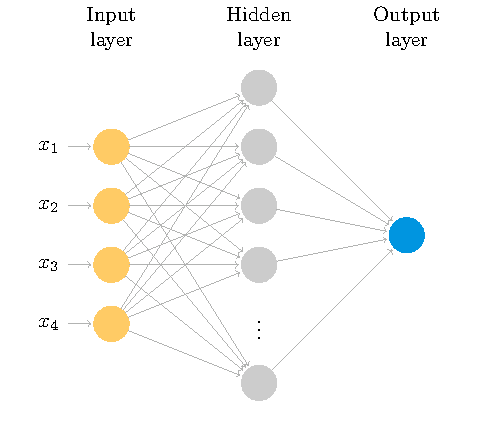
\includegraphics[clip=true]{neuralnet/neuralnet.pdf}
  \end{figure}
\end{frame}

\begin{frame}{O problema de seleção de características}
  A seleção de características é uma etapa da seleção de modelos. Ela
  deve escolher quais são as melhores características para se considerar
  no modelo.
  \pause
  \begin{mydefinition}
    Dado um conjunto $S$ de características e uma função 
    de custo $c$, ache o subconjunto de 
    $X \in \powerset(S)$ tal que $c (X)$ é mínimo.
  \end{mydefinition}
\end{frame}


\begin{frame}{O problema de seleção de características}
  Podemos representar um conjunto $X$ de características por um vetor
  de bits que chamamos de \alert{vetor característico}. \\
  %\pause
  %Assuma que o conjunto $S$ tem uma ordem $S = \langle s_1, s_2, ..., s_n \rangle$.
  %Então, se o conjunto $X$ possui a i-ésima característica de $S$, então
  %o i-ésimo bit do vetor característico deve estar ligado.
  \pause
  \vspace{1em}
  Por exemplo, se $S = \{s_1, s_2, s_3\}$ e $X = \{s_1, s_3\}$
  então o vetor característico de $X$ é $101$.
\end{frame}

\begin{frame}{O espaço de busca}
  Os algoritmos estudados neste trabalho representam o espaço de busca
  com o reticulado Booleano $(\powerset(S), \subseteq)$.
  \begin{figure}
    \centering
    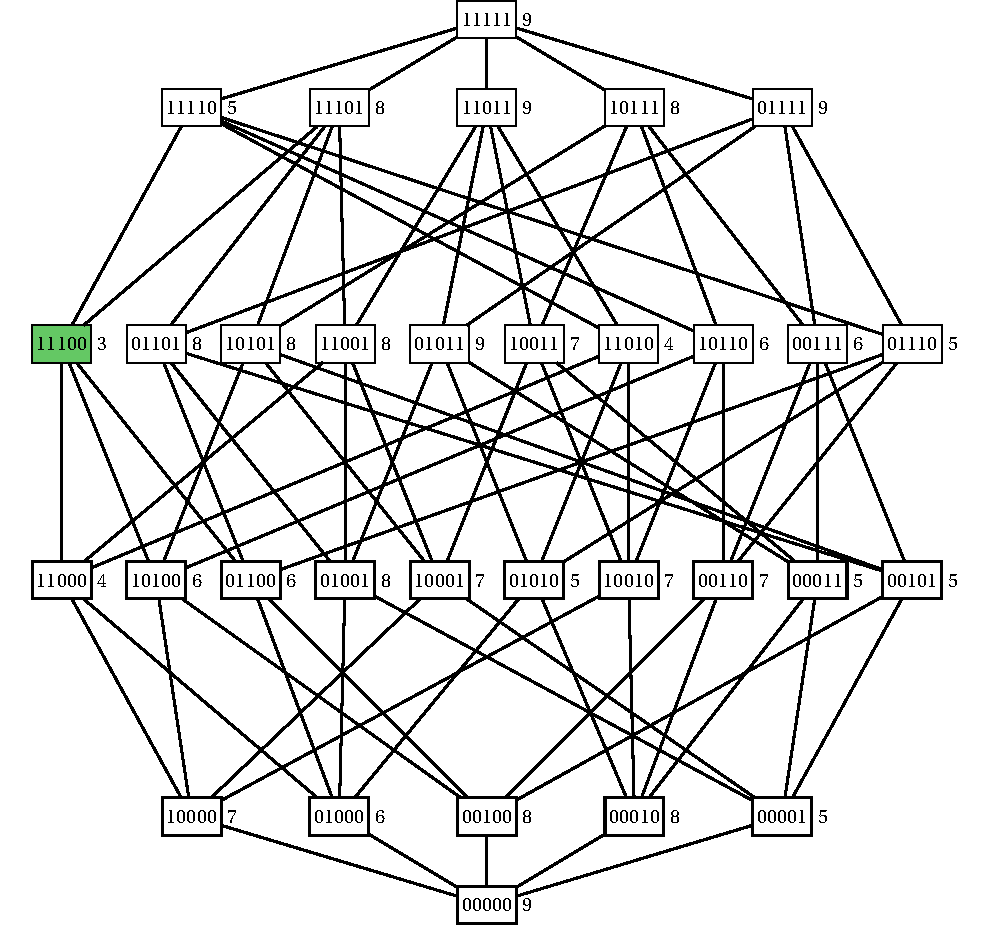
\includegraphics[clip=true, width=.6\textwidth]{lattice/Boolean_lattice.pdf}
  \end{figure}
\end{frame}

\begin{frame}{O espaço de busca}
  Chamamos de \alert{cadeia} uma sequência de conjuntos adjacentes 
  $X_1, X_2, \dots, X_n$ tal que $X_1 \subseteq X_2 \subseteq \dots \subseteq X_n$. 
  \pause
  \begin{figure}
    \centering
    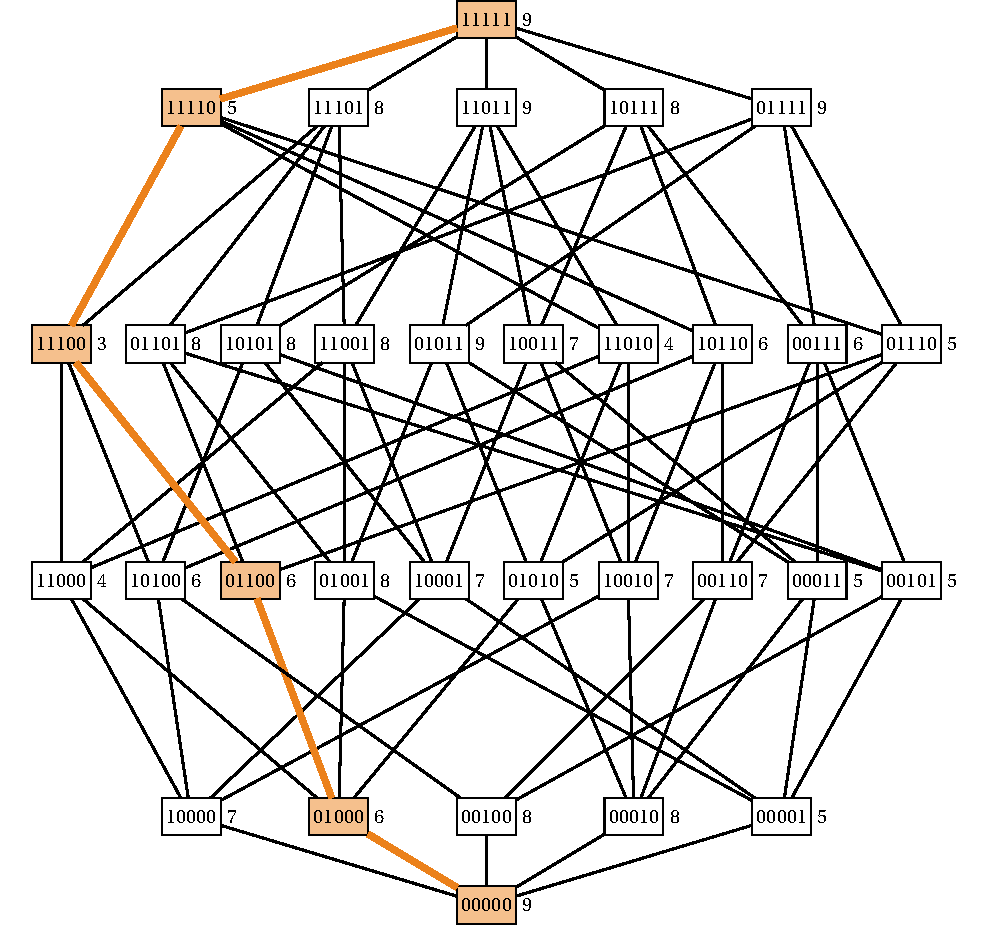
\includegraphics[clip=true, width=.6\textwidth]{lattice/chain.pdf}
  \end{figure}
\end{frame}

\begin{frame}{A função de custo}
  A função de custo $c$ deve refletir a qualidade de um conjunto de 
  características $X$ a ser usado no modelo.\\
  \pause
  \vspace{1em}
  Nestas funções, um fenômeno conhecido em aprendizado de máquina aparece.
  A função descreve curvas em U nas cadeias do reticulado.
  \begin{figure}[ht]
    \centering
    \begin{tabular}{c c}
    \subfigure {\scalebox{.4}{
        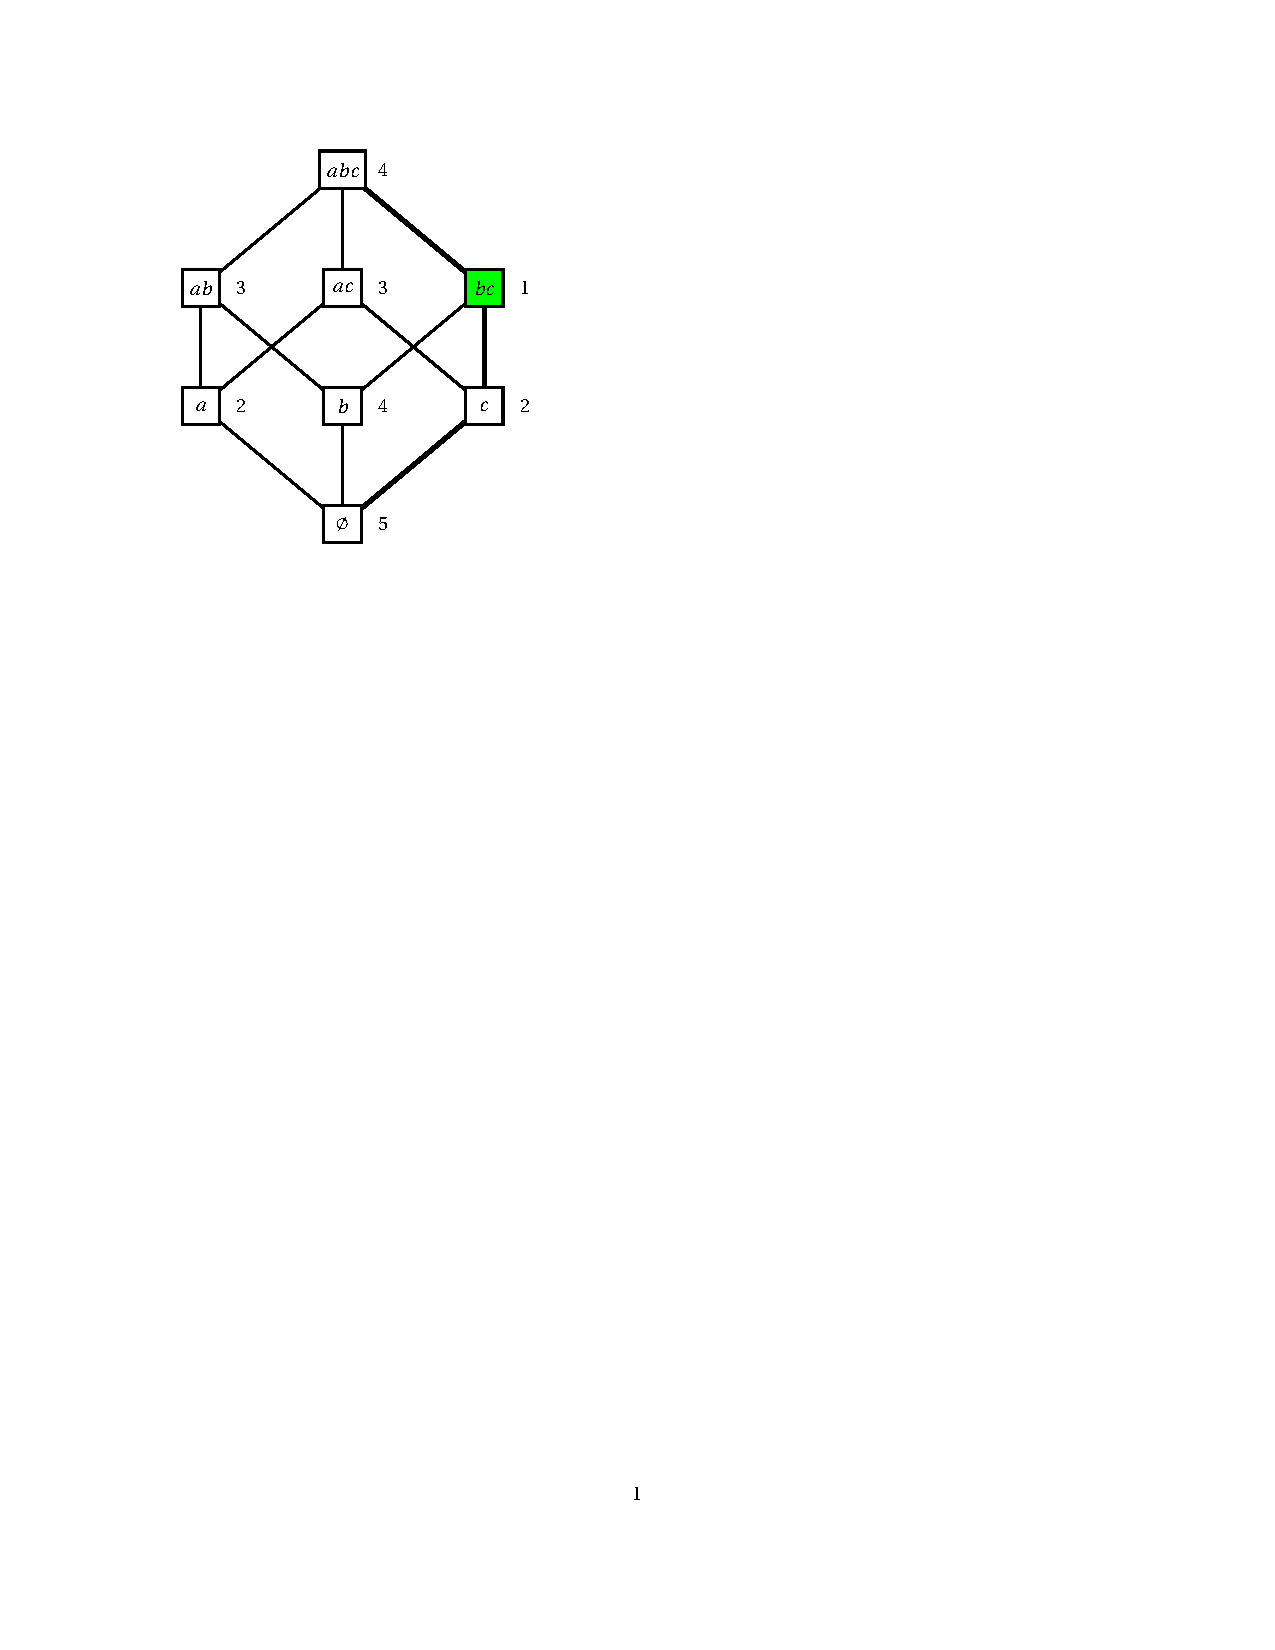
\includegraphics[clip=true, trim={3cm 18cm 13cm 2cm}]{intro/example_lattice_3.pdf}}
    \label{fig:intro:lattice} }
    & 
    \subfigure {\scalebox{.15}{
        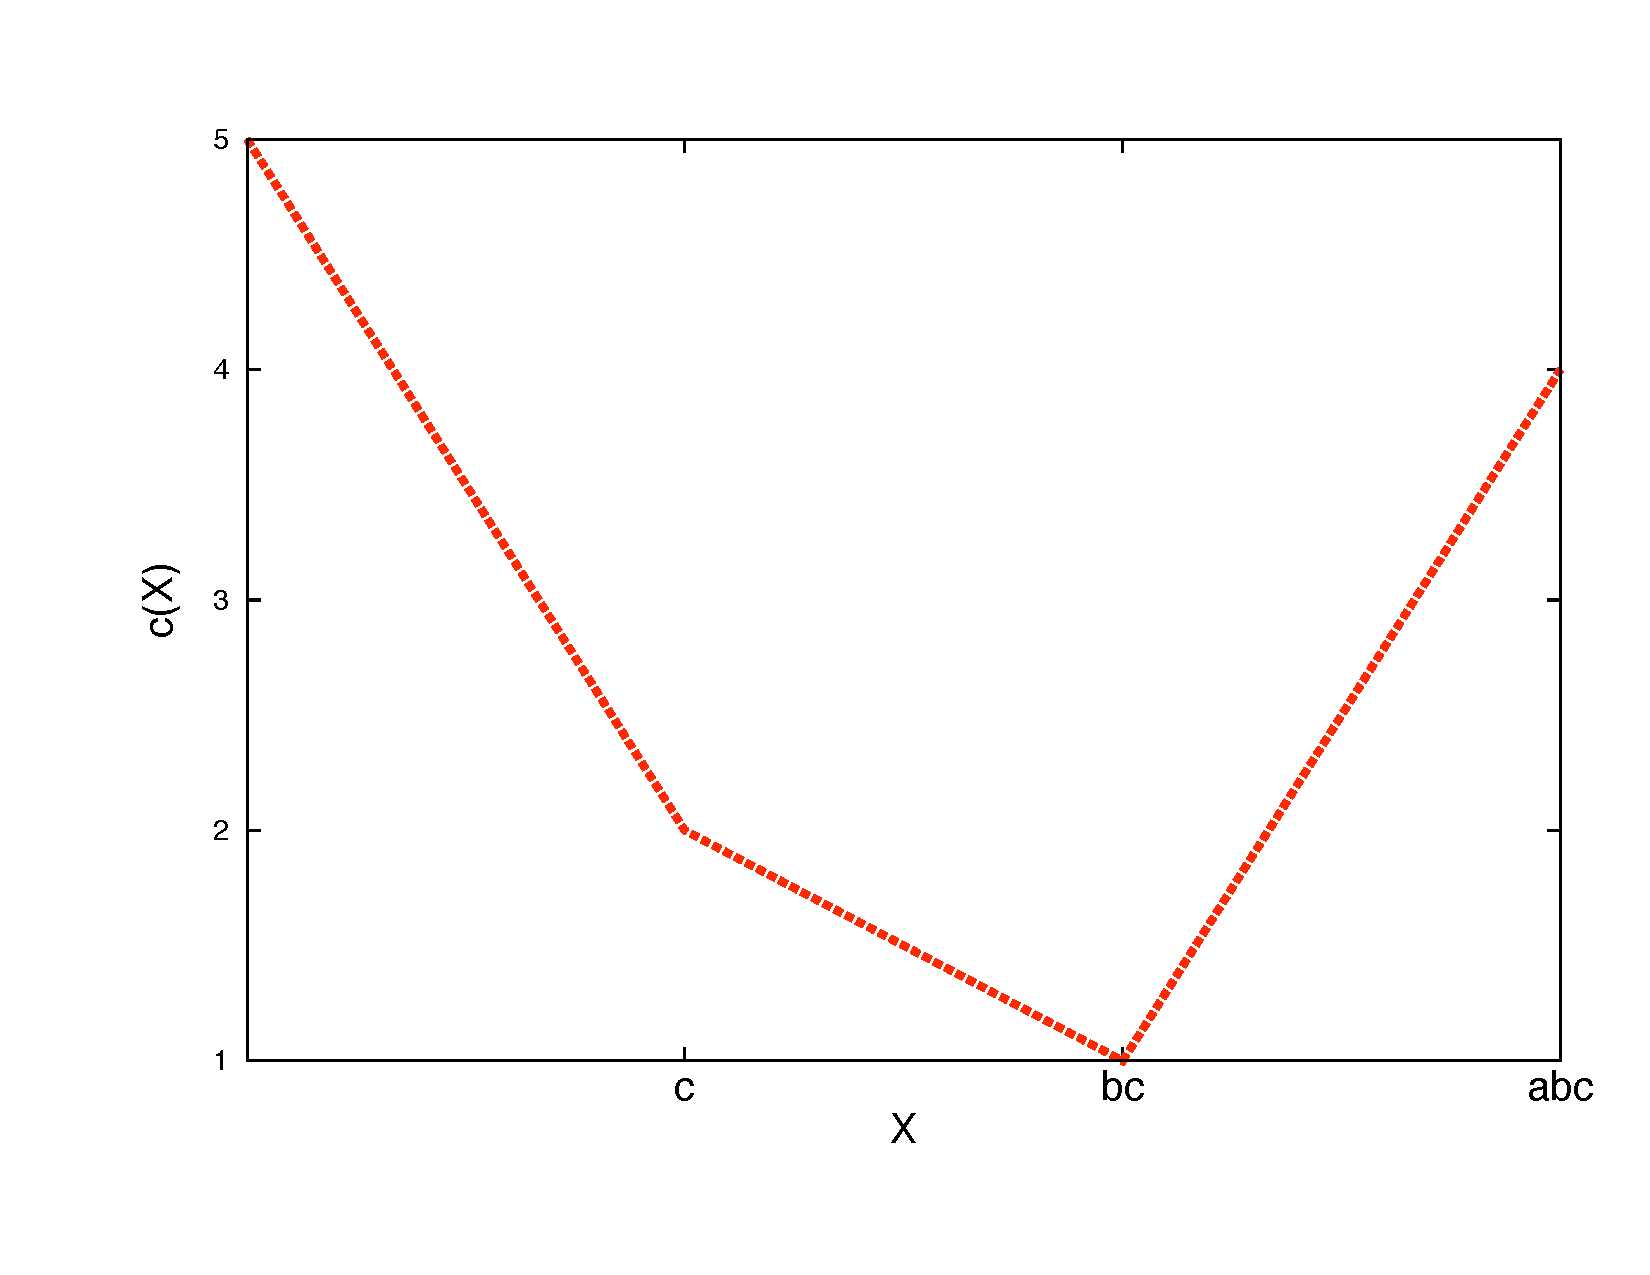
\includegraphics[clip=true, trim={1cm 0cm 1cm 2cm}]{intro/example_lattice_chain_3.pdf}}
    \label{fig:intro:chain} }
    \end{tabular}
\end{figure}
\end{frame}

\begin{frame}{Funções decomponíveis em curvas U}
\begin{mydefinition}\label{fund_concepts:ushape}
Uma função de custo $c$ é dita {\bf \em decomponível em curvas U} se
para toda cadeia maximal $X_1, ..., X_l$, $c(X_j) \leq max \{c (X_i),
c (X_k)\}$ sempre que $X_i \subseteq X_j \subseteq X_k$, $i, j, k \in 
\{1, ..., l\}$.
\end{mydefinition}
\end{frame}


\begin{frame}{O problema U-curve}
\begin{mydefinition}[Problema U-Curve]
Dados um conjunto finito e não-vazio $S$ e uma função de custo $c$ 
decomponível em curvas U, encontrar um subconjunto $X \in \powerset (S)$ 
tal que $c(X)$ é mínimo.
\end{mydefinition}
\end{frame}

\section{Algoritmos baseados em florestas}
\begin{frame}{O algoritmo \algname{U-Curve-Branch-and-Bound}}
O algoritmo \algname{U-Curve-Branch-and-Bound} (\algname{UBB}) organiza
o espaço de busca em uma árvore.
\begin{figure}[!ht]
  \centering 
  \begin{tabular}{c c}
    \subfigure {\scalebox{0.3}{
     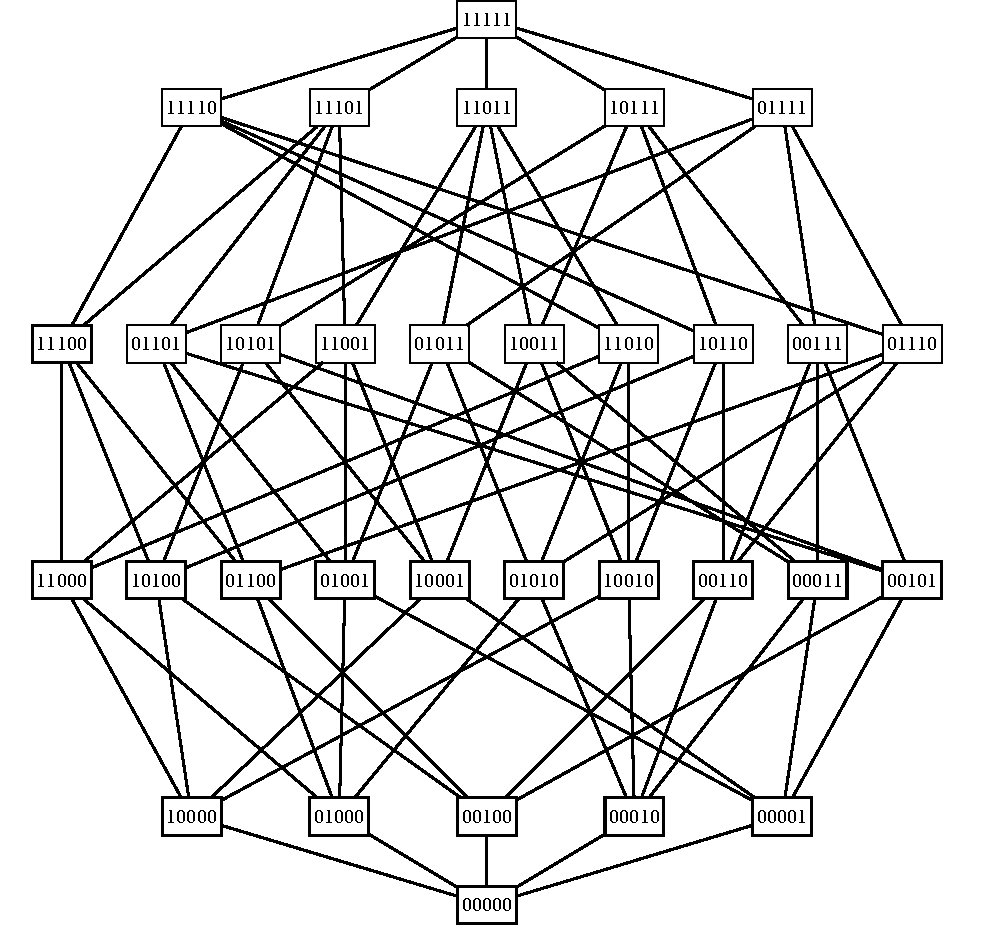
\includegraphics[clip=true]{pfs/ubb/full_lattice.pdf}}
     \label{fig:ubb:full} }
    & 
    \subfigure {\scalebox{.3}{
    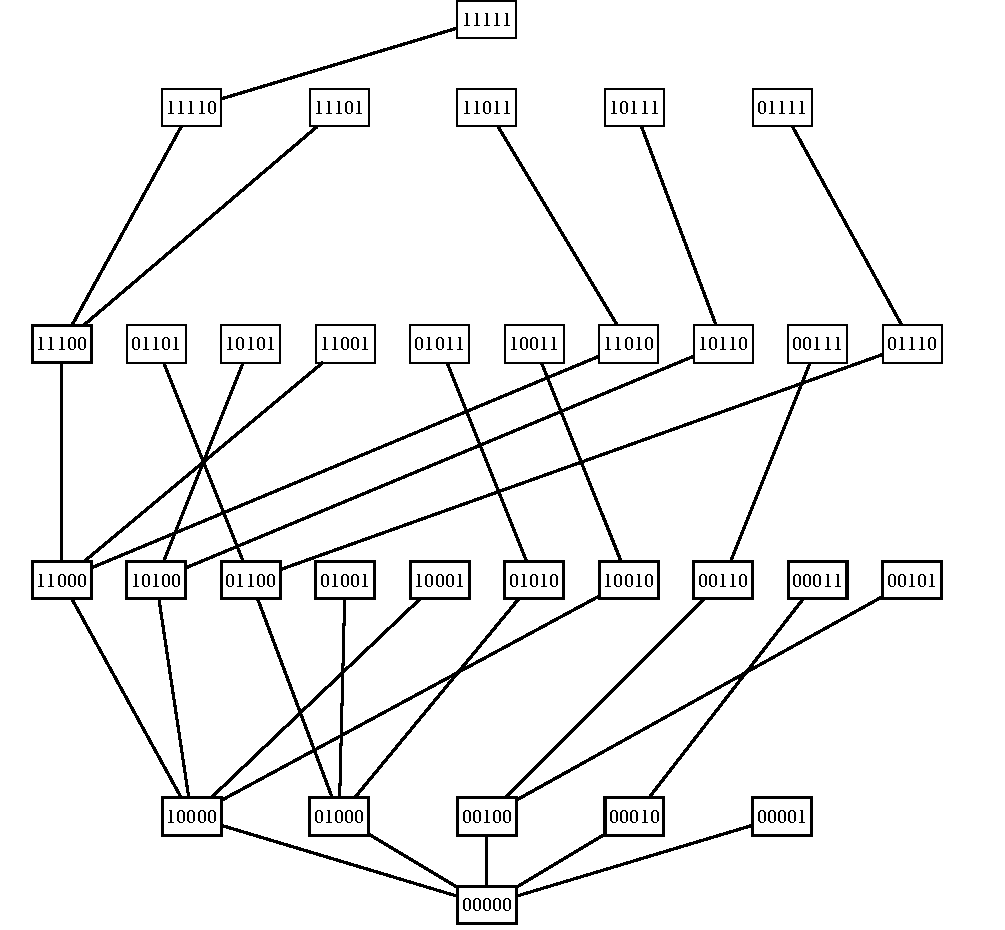
\includegraphics[clip=true]{pfs/ubb/ubb_tree.pdf}}
    \label{fig:ubb:tree} }
  \end{tabular}
\end{figure}  
\end{frame}

\begin{frame}{O algoritmo \algname{U-Curve-Branch-and-Bound}}
Este algoritmo busca o mínimo global ramificando na árvore como em uma
busca em profundidade e faz podas sempre que o custo aumenta.
\begin{figure}[!ht]
  \centering 
  \begin{tabular}{c c}
    \subfigure {\scalebox{0.3}{
     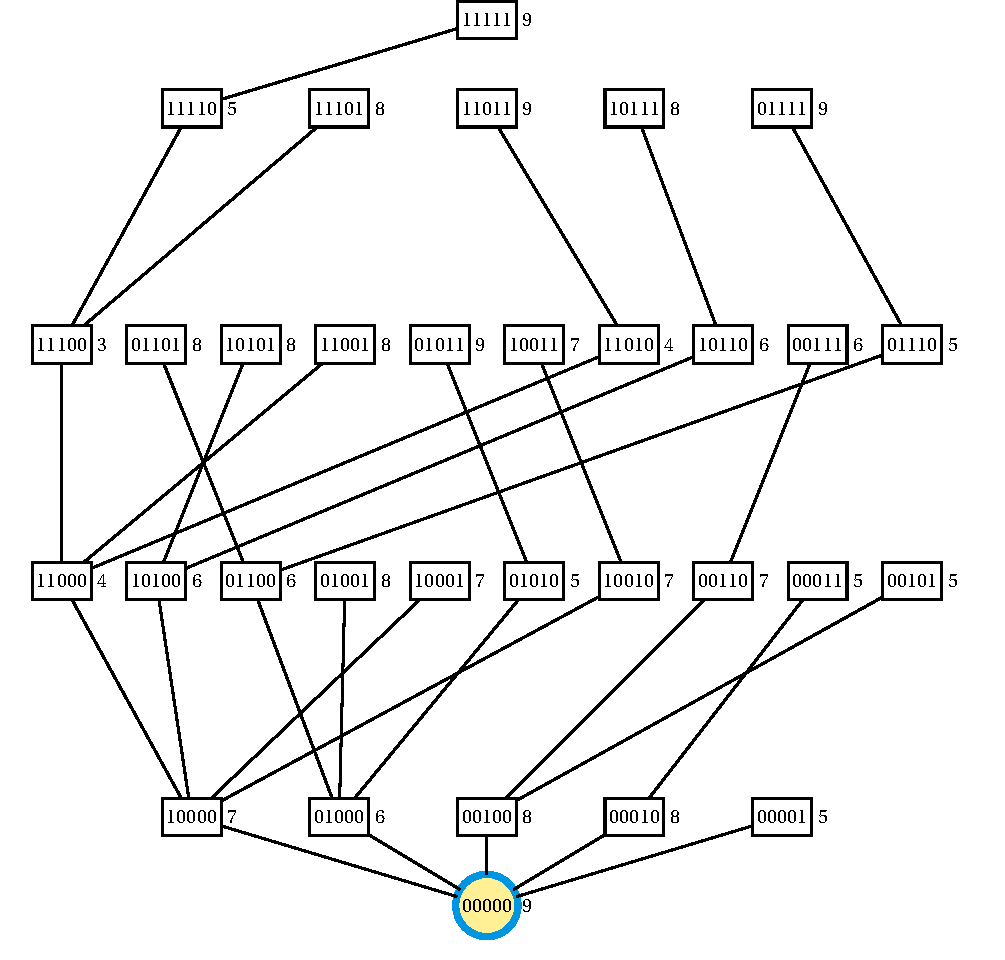
\includegraphics[clip=true]{pfs/ubb_run/b.pdf}}
     \label{fig:ubb:full} }
    & 
    \pause
    \subfigure {\scalebox{.3}{
    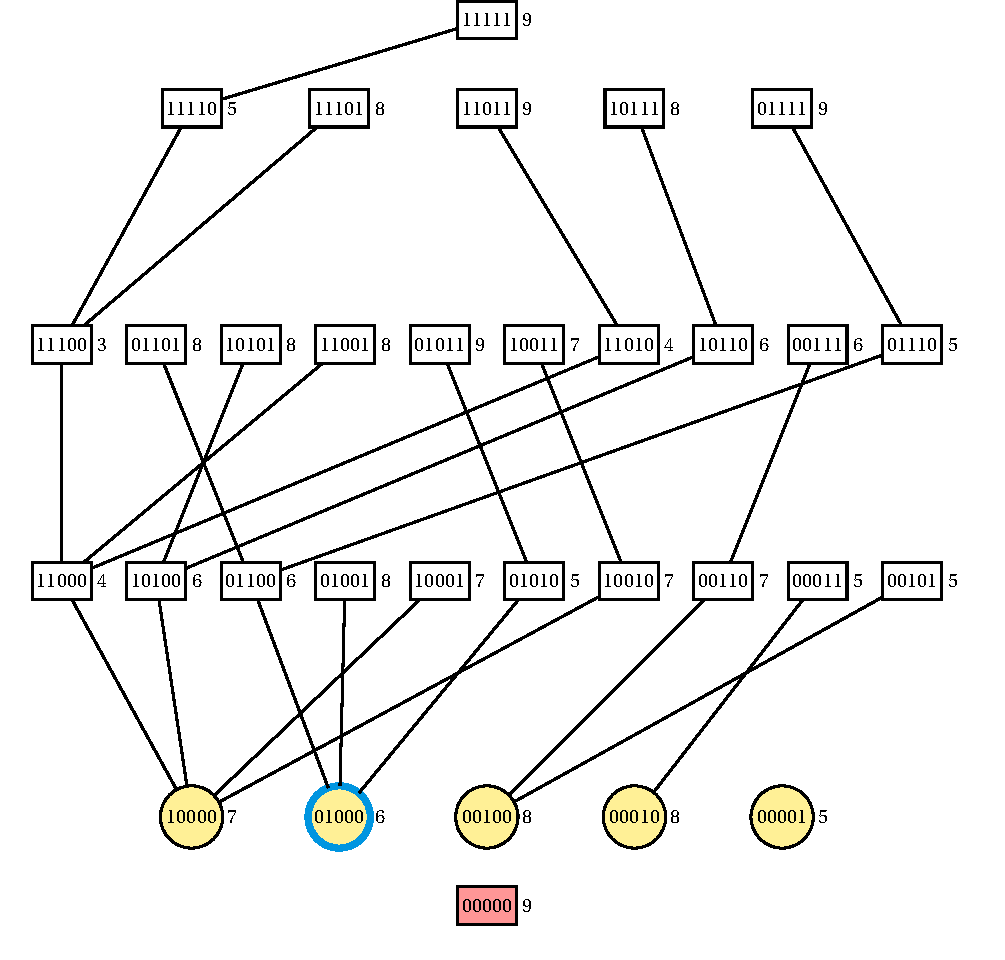
\includegraphics[clip=true]{pfs/ubb_run/c.pdf}}
    \label{fig:ubb:tree} }
  \end{tabular}
\end{figure}  
\end{frame}

\begin{frame}{O algoritmo \algname{U-Curve-Branch-and-Bound}}
\begin{figure}[!ht]
  \centering 
  \begin{tabular}{c c}
    \subfigure {\scalebox{0.3}{
     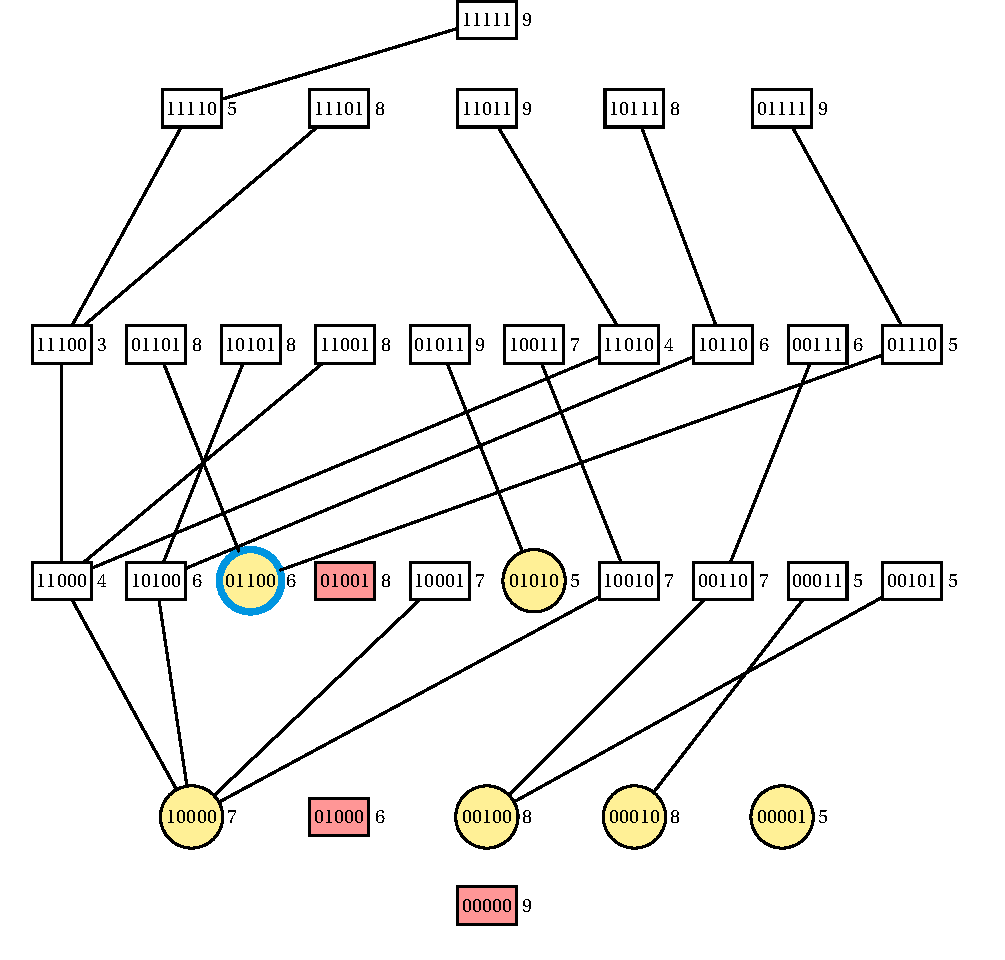
\includegraphics[clip=true]{pfs/ubb_run/d.pdf}}
     \label{fig:ubb:full} }
    \pause
    & 
    \subfigure {\scalebox{.3}{
    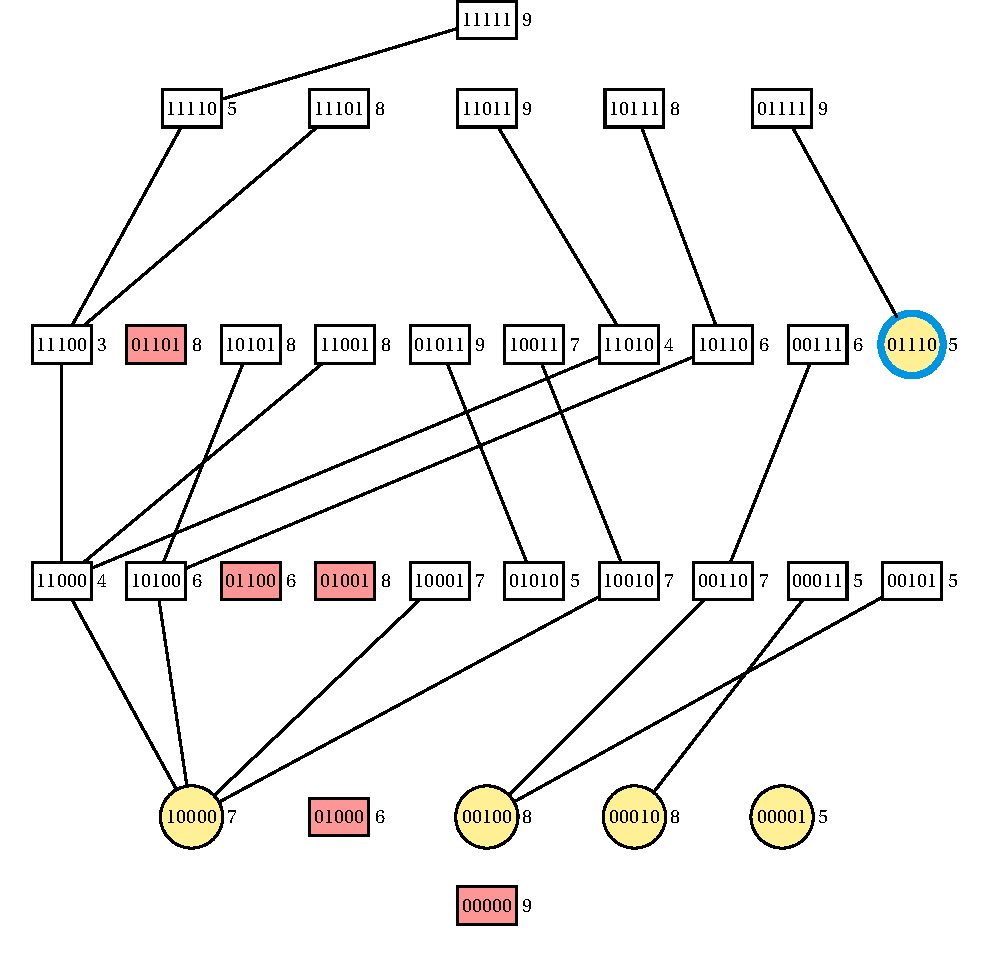
\includegraphics[clip=true]{pfs/ubb_run/e.pdf}}
    \label{fig:ubb:tree} }
  \end{tabular}
\end{figure}  
\pause
Note que se a condição de poda nunca é verdadeira, então o espaço
de busca inteiro é percorrido.
\end{frame}

\begin{frame}{O algoritmo \algname{Poset-Forest-Search}}
  Solução: percorrer o espaço de busca em duas direções.
  \pause
  %\vspace{1em}
  
  O algoritmo \algname{Poset-Fores-Search} (\algname{PFS}) pode fazer
  isso porque decompõe o espaço em duas árvores.
  \begin{figure}[!ht]
  \centering 
  \begin{tabular}{c c}
    \subfigure {\scalebox{0.28}{
     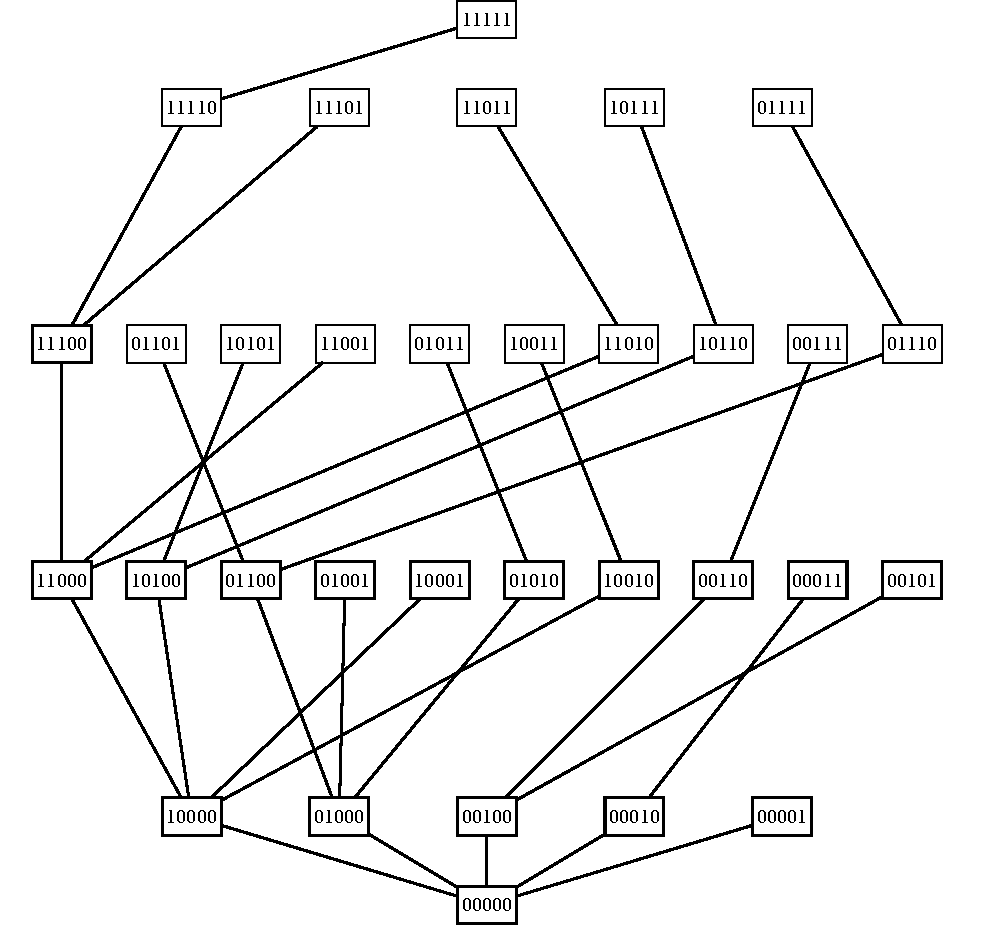
\includegraphics[clip=true]{pfs/pfs/lower_tree.pdf}}
     \label{fig:ubb:full} }
    \pause
    & 
    \subfigure {\scalebox{.28}{
    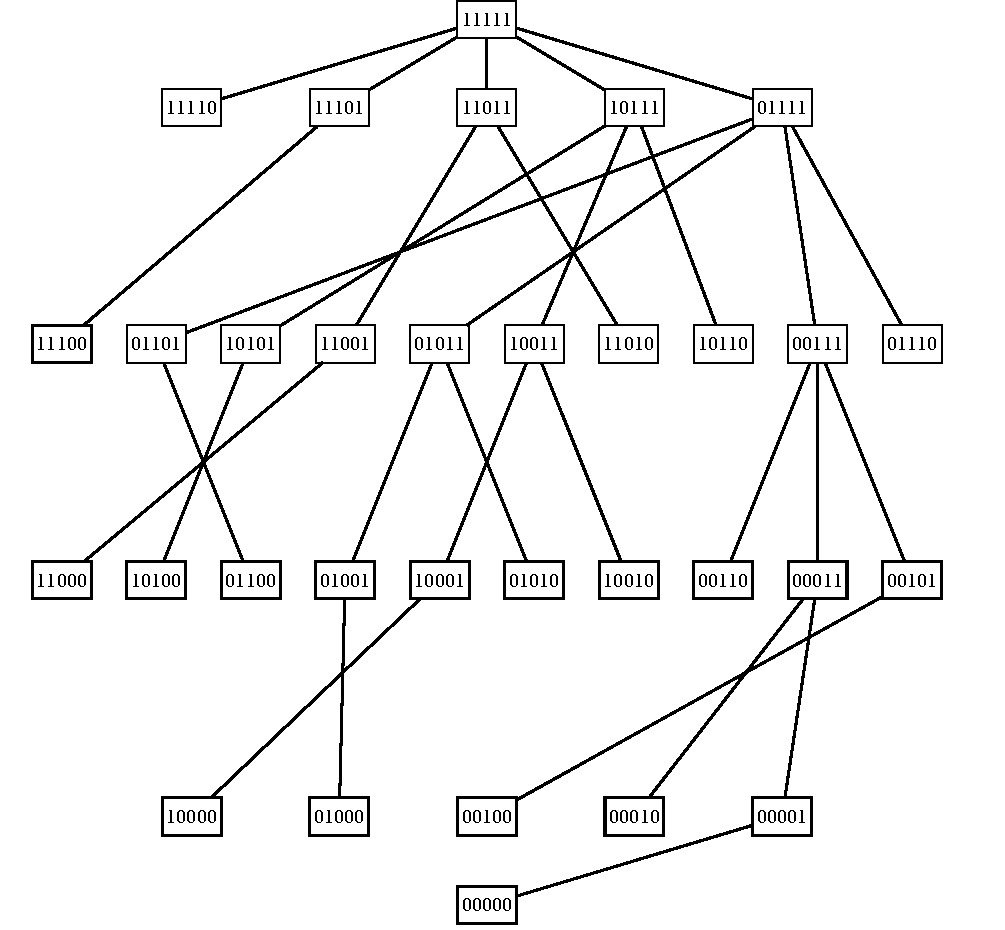
\includegraphics[clip=true]{pfs/pfs/upper_tree.pdf}}
    \label{fig:ubb:tree} }
  \end{tabular}
  \end{figure}  
\end{frame}

\begin{frame}{O algoritmo \algname{Poset-Forest-Search}}
  Problema: agora é necessário manter as duas árvores equivalentes,
  ou seja, representando o mesmo espaço de busca.
  \begin{figure}[!ht]
  \centering 
  \begin{tabular}{c c}
    \subfigure {\scalebox{0.28}{
     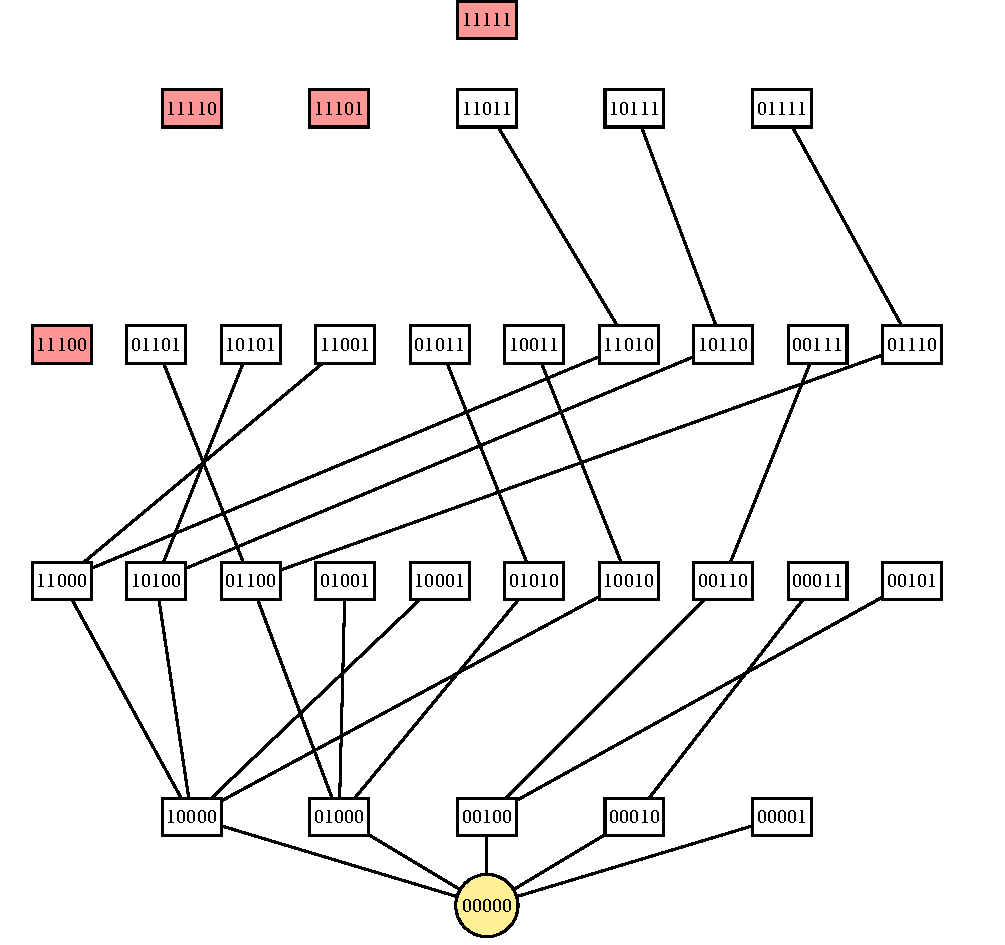
\includegraphics[clip=true]{pfs/pfs/forest/lower_tree.pdf}}
     \label{fig:ubb:full} }
    & 
    \pause
    \subfigure {\scalebox{.28}{
    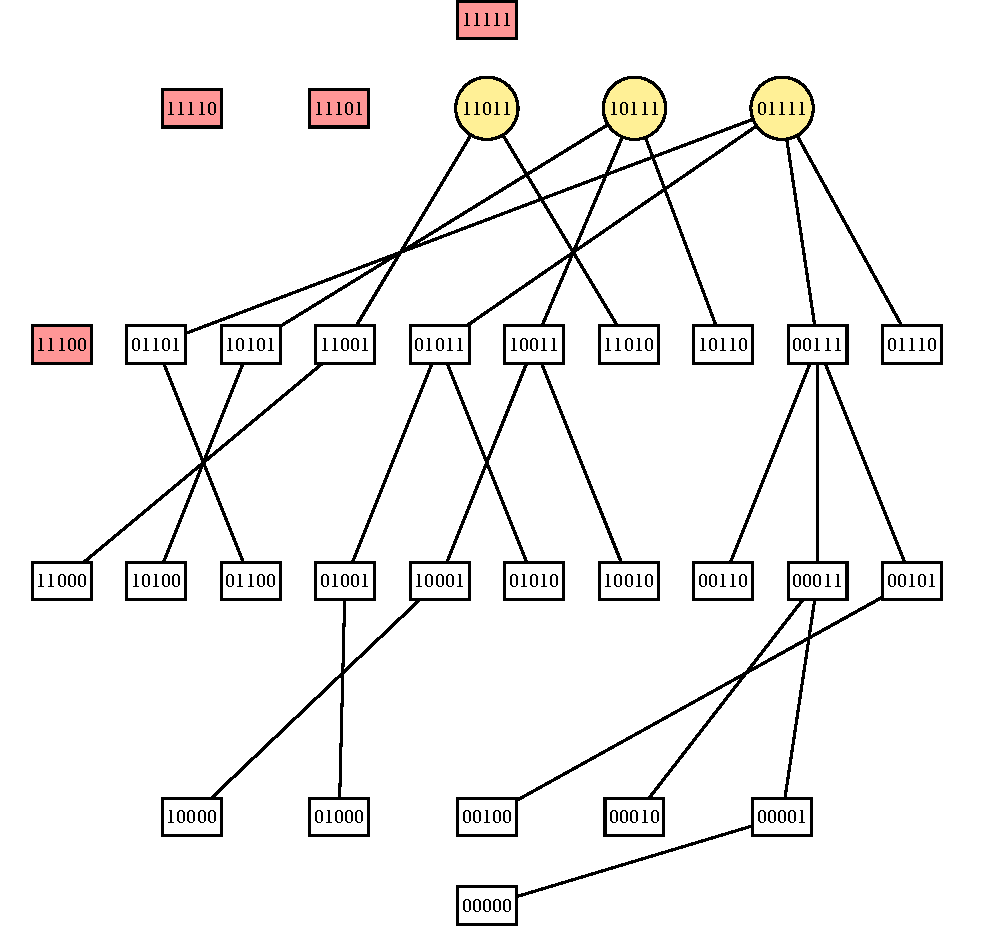
\includegraphics[clip=true]{pfs/pfs/forest/upper_tree.pdf}}
    \label{fig:ubb:tree} }
  \end{tabular}
  \end{figure}  
\end{frame}

\begin{frame}{O algoritmo \algname{Poset-Forest-Search}}
Podemos resumir o funcionamento do \algname{PFS} aos seguintes passos:
\pause
\begin{itemize}
  \item{Escolher uma direção de percorrimento}
  \pause
  \item{Percorrer uma cadeia da floresta escolhida}
  \pause
  \item{Sempre que a condição de poda for verdadeira:}
  \pause
    \begin{itemize}
    \item{Podar a floresta de percorrimento}
    \pause
    \item{Atualizar a floresta dual}
    \pause
    \end{itemize}
\end{itemize}
\end{frame}


%----------------------------------------------------------------------
\section{Melhoramentos ao \algname{Poset-Forest-Search}}


\begin{frame}{Melhoramentos na implementação atual do \algname{PFS}}
  O algoritmo implementado por Marcelo possui pontos que podiam ser
  explorados para se ter melhor desempenho computacional.
\end{frame}


\begin{frame}{Mudanças na escolha de raízes}
A implementação de Marcelo escolhia \alert{arbitrariamente} como raiz de
percorrimento a primeira quando ordenadas lexicograficamente.
\vspace{2em}\\
\pause
Propomos duas estratégias de escolhas:
\begin{itemize}
  \item{escolha aleatória e uniforme entre raízes;}
  \pause
  \item{escolha da raiz com maior sub-árvore.}
\end{itemize}
\end{frame}


\begin{frame}{Resultados da mudança de escolha de raízes}
Chamamos a variação do \algname{PFS} que escolhe raízes de maneira 
aleatória e identicamente provável de \algname{PFS-RAND}.
\pause
\begin{table}
\centering
\footnotesize
\label{tab:pfsrand_vs_pfs}
\resizebox{\columnwidth}{!}{%
\begin{tabular}{cc c cc c cc}
\toprule
\multicolumn{2}{c}{Instância} & \phantom{} & \multicolumn{2}{c}{Tempo de execução médio (s)}  & \phantom{} & \multicolumn{2}{c}{Número médio de cálculos de custo}\\
\cline{1-2}\cline{4-5}\cline{7-8}\\
$|S|$ & $2^{|S|}$ && \algname{PFS} & \algname{PFS\_RAND} && \algname{PFS} & \algname{PFS\_RAND} \\
10 &    1024 &&  0.013 $\pm$ 0.003 & 0.014 $\pm$ 0.003 &&   590.8 $\pm$ 198.5 & 599.5 $\pm$ 177.5 \\
11 &    2048 &&  0.019 $\pm$ 0.004 & 0.022 $\pm$ 0.007 &&   1114.8 $\pm$ 331.3 & 1090.1 $\pm$ 350.3 \\
12 &    4096 &&  0.029 $\pm$ 0.008 & 0.036 $\pm$ 0.013 &&   1848.6 $\pm$ 600.8 & 1835.7 $\pm$ 683.0 \\
13 &    8192 &&  0.060 $\pm$ 0.018 & 0.090 $\pm$ 0.039 &&   4314.4 $\pm$ 1496.4 & 4201.1 $\pm$ 1580.7 \\
14 &   16384 &&  0.100 $\pm$ 0.041 & 0.191 $\pm$ 0.110 &&   7323.4 $\pm$ 3318.9 & 7333.8 $\pm$ 3161.0 \\
15 &   32768 &&  0.180 $\pm$ 0.076 & 0.453 $\pm$ 0.311 &&   12958.1 $\pm$ 5654.0 & 12807.5 $\pm$ 5753.7 \\
16 &   65536 &&  0.406 $\pm$ 0.185 & 1.715 $\pm$ 1.400 &&   27573.8 $\pm$ 12459.5 & 27036.9 $\pm$ 12687.5 \\
17 &  131072 &&  0.717 $\pm$ 0.397 & 5.416 $\pm$ 5.266 &&   48176.2 $\pm$ 26938.3 & 47852.1 $\pm$ 26427.6 \\
18 &  262144 &&  1.325 $\pm$ 0.754 & 15.890 $\pm$ 17.726 &&   84417.9 $\pm$ 48587.7 & 84025.0 $\pm$ 48882.4 \\
19 &  524288 &&  2.771 $\pm$ 1.603 & 69.600 $\pm$ 82.342 &&   167659.1 $\pm$ 99686.7 & 164612.1 $\pm$ 102018.3 \\
\bottomrule
\end{tabular}%
}
\end{table}
\end{frame}


\begin{frame}{Resultados da mudança de escolha de raízes}
Chamamos a variação do \algname{PFS} que escolhe as raízes com maior
sub-árvore de \algname{PFS-LEFTMOST}.
\pause
\begin{table}
\centering
\resizebox{\columnwidth}{!}{%
\begin{tabular}{cc c cc c cc}
\toprule
\multicolumn{2}{c}{Instância} & \phantom{} & \multicolumn{2}{c}{Tempo de execução médio (s)}  & \phantom{} & \multicolumn{2}{c}{Número médio de cálculos de custo}\\
\cline{1-2}\cline{4-5}\cline{7-8}\\
$|S|$ & $2^{|S|}$ && \algname{PFS} & \algname{PFS\_LEFTMOST} && \algname{PFS} & \algname{PFS\_LEFTMOST} \\
10 &    1024 &&  0.013 $\pm$ 0.002 & 0.023 $\pm$ 0.004 &&  606.1 $\pm$ 133.5 & 665.0 $\pm$ 165.8 \\
11 &    2048 &&  0.020 $\pm$ 0.004 & 0.042 $\pm$ 0.010 &&  1122.1 $\pm$ 351.2 & 1316.6 $\pm$ 382.2 \\
12 &    4096 &&  0.032 $\pm$ 0.008 & 0.078 $\pm$ 0.024 &&  2183.7 $\pm$ 733.2 & 2515.8 $\pm$ 871.3 \\
13 &    8192 &&  0.054 $\pm$ 0.017 & 0.160 $\pm$ 0.061 &&  3887.7 $\pm$ 1389.9 & 4716.8 $\pm$ 1777.8 \\
14 &   16384 &&  0.107 $\pm$ 0.034 & 0.345 $\pm$ 0.133 &&  7851.2 $\pm$ 2793.0 & 9506.8 $\pm$ 3673.9 \\
15 &   32768 &&  0.196 $\pm$ 0.085 & 0.672 $\pm$ 0.274 &&  13780.3 $\pm$ 6049.9 & 17071.6 $\pm$ 7005.1 \\
16 &   65536 &&  0.348 $\pm$ 0.189 & 1.271 $\pm$ 0.661 &&  24106.5 $\pm$ 13159.9 & 30055.6 $\pm$ 15363.6 \\
17 &  131072 &&  0.785 $\pm$ 0.361 & 3.137 $\pm$ 1.476 &&  52369.0 $\pm$ 24751.2 & 67585.6 $\pm$ 30978.4 \\
18 &  262144 &&  1.445 $\pm$ 0.657 & 6.146 $\pm$ 3.032 &&  92095.9 $\pm$ 42566.6 & 120635.7 $\pm$ 58039.0 \\
19 &  524288 &&  3.298 $\pm$ 1.883 & 13.881 $\pm$ 7.595 &&  199151.0 $\pm$ 112167.8 & 256078.6 $\pm$ 135958.4 \\
\bottomrule 
\end{tabular}%
}
\end{table}
\end{frame}


\begin{frame}{Melhoramentos na estrutura de armazenamento de raízes}
  Mudamos a implementação de Marcelo para usar diagramas de decisão
  binários ordenados (OBDDs).
  \pause
  \begin{figure}[]
  \centering 
  \begin{tabular}{c c}
    \subfigure {\scalebox{.5}{
     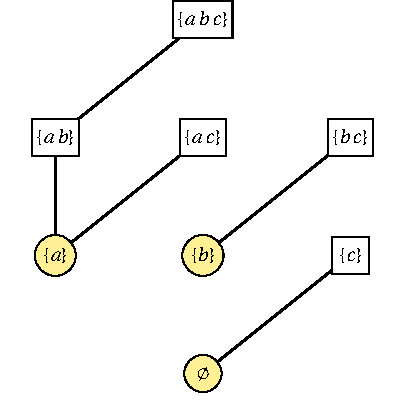
\includegraphics[clip=true]{pfs/obdd/lattice.pdf}}
     \label{fig:pfs:obdd:A} }
      & 
      \subfigure {\scalebox{.65}{
    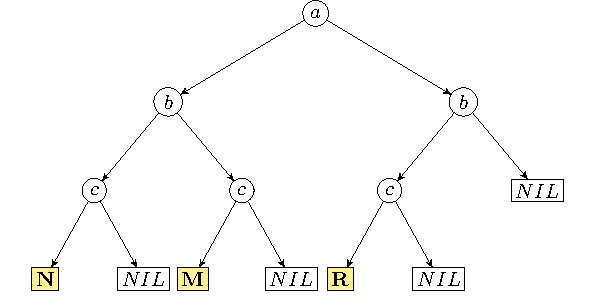
\includegraphics[clip=true]{pfs/obdd/obdd.pdf}}
    \label{fig:pfs:obdd:B} }
  \end{tabular}
  \end{figure}
\end{frame}


\begin{frame}{Resultados da mudança de estrutura para armazenamento de raízes}
Chamamos de \algname{OPFS} o algoritmo que usa OBDDs para armazenamento
de raízes.
\begin{table}
\centering
\resizebox{\columnwidth}{!}{
\begin{tabular}{cc c cc c cc}
\toprule
\multicolumn{2}{c}{Instância} & \phantom{} & \multicolumn{2}{c}{Tempo de execução médio (s)}  & \phantom{} & \multicolumn{2}{c}{Número médio de cálculos de custo}\\
\cline{1-2}\cline{4-5}\cline{7-8}\\
$|S|$ & $2^{|S|}$ && \algname{PFS} & \algname{OPFS} && \algname{PFS} & \algname{OPFS} \\
10 &    1024 &&  0.013 $\pm$ 0.003 & 0.018 $\pm$ 0.003 &&  598.0 $\pm$ 192.8 & 635.5 $\pm$ 171.9 \\
11 &    2048 &&  0.020 $\pm$ 0.004 & 0.029 $\pm$ 0.007 &&  1152.1 $\pm$ 314.7 & 1117.9 $\pm$ 336.4 \\
12 &    4096 &&  0.031 $\pm$ 0.010 & 0.049 $\pm$ 0.013 &&  2024.1 $\pm$ 751.6 & 2048.2 $\pm$ 700.9 \\
13 &    8192 &&  0.057 $\pm$ 0.017 & 0.097 $\pm$ 0.033 &&  3996.3 $\pm$ 1431.6 & 3973.4 $\pm$ 1462.6 \\
14 &   16384 &&  0.094 $\pm$ 0.038 & 0.171 $\pm$ 0.063 &&  6634.8 $\pm$ 2944.0 & 6906.5 $\pm$ 2786.5 \\
15 &   32768 &&  0.182 $\pm$ 0.079 & 0.323 $\pm$ 0.156 &&  13140.1 $\pm$ 6020.6 & 12711.2 $\pm$ 6319.7 \\
16 &   65536 &&  0.370 $\pm$ 0.169 & 0.660 $\pm$ 0.314 &&  25658.2 $\pm$ 11606.7 & 25303.4 $\pm$ 12169.5 \\
17 &  131072 &&  0.819 $\pm$ 0.370 & 1.480 $\pm$ 0.665 &&  53344.9 $\pm$ 24350.4 & 53217.2 $\pm$ 24154.5 \\
18 &  262144 &&  1.515 $\pm$ 0.905 & 2.736 $\pm$ 1.626 &&  94677.6 $\pm$ 54496.3 & 94079.4 $\pm$ 55435.6 \\
19 &  524288 &&  2.612 $\pm$ 1.869 & 4.818 $\pm$ 3.355 &&  156150.5 $\pm$ 107369.8 & 156021.8 $\pm$ 107516.8 \\
20 & 1048576 &&  6.085 $\pm$ 3.900 & 11.550 $\pm$ 7.661 &&  344144.1 $\pm$ 212627.1 & 343229.2 $\pm$ 212624.4 \\
% 21 & 2097152 &&  11.416 $\pm$ 8.296 & 21.818 $\pm$ 16.269 &&  616936.2 $\pm$ 436491.2 & 613526.2 $\pm$ 438580.0 \\
% 22 & 4194304 &&  19.950 $\pm$ 17.799 & 42.112 $\pm$ 45.109 &&  960842.2 $\pm$ 785137.2 & 959905.4 $\pm$ 783257.3 \\
% 23 & 8388608 &&  42.792 $\pm$ 35.622 & 87.262 $\pm$ 90.579 &&  2053472.4 $\pm$ 1690882.1 & 2060184.5 $\pm$ 1682011.0 \\
% 24 & 16777216 &&  85.646 $\pm$ 79.186 & 149.567 $\pm$ 108.104 &&  4080290.8 $\pm$ 3166258.4 & 4100480.6 $\pm$ 3141423.9 \\
\bottomrule 
\end{tabular}%
}
\end{table}
\end{frame}


\begin{frame}{Paralelização do \algname{PFS}}
Implementamos também uma versão paralela do algoritmo \algname{PFS}.
\vspace{1em}
\pause\\

Entretanto, a etapa de atualização da floresta dual é complicada e pode 
gerar condições de corrida, o que deixou a paralelização complicada.
\end{frame}

\begin{frame}{O algoritmo \algname{UBB-PFS}}
Este algoritmo é uma nova alternativa paralela que é dividida em duas
partes:
\vspace{1em}
\pause\\
\begin{itemize}
  \item{Percorrimento sequencial: idêntico ao \algname{UBB} deve criar
    sub-árvores no espaço enquanto faz uma ramificação do tipo
    busca em profundidade.}
  \pause
  \item{Solução em paralelo: cada sub-árvore gerada na etapa de 
    ramificação deve ser resolvida por uma chamada do \algname{PFS}.}
\end{itemize}
\end{frame}


\begin{frame}{Resultados do \algname{UBB-PFS}}
O \algname{UBB-PFS} foi mais rápido do que o \algname{PFS}.
\begin{table}
\centering
\footnotesize
\resizebox{\columnwidth}{!}{%
\begin{tabular}{cc c ccc}
\toprule
\multicolumn{2}{c}{Instância} & \phantom{} & \multicolumn{3}{c}{Tempo de execução médio (s)}\\
\cline{1-2}\cline{4-6}\\
$|S|$ & $2^{|S|}$ && UBB & PFS & UBB-PFS  \\
%10 &    1024 &&  0.006 $\pm$ 0.001 & 0.011 $\pm$ 0.002 & 0.023 $\pm$ 0.004 \\
%11 &    2048 &&  0.007 $\pm$ 0.001 & 0.017 $\pm$ 0.004 & 0.026 $\pm$ 0.004 \\
%12 &    4096 &&  0.010 $\pm$ 0.003 & 0.029 $\pm$ 0.009 & 0.034 $\pm$ 0.006 \\
%13 &    8192 &&  0.013 $\pm$ 0.006 & 0.047 $\pm$ 0.016 & 0.044 $\pm$ 0.011 \\
%14 &   16384 &&  0.024 $\pm$ 0.013 & 0.094 $\pm$ 0.034 & 0.068 $\pm$ 0.023 \\
%15 &   32768 &&  0.043 $\pm$ 0.026 & 0.186 $\pm$ 0.074 & 0.113 $\pm$ 0.042 \\
%16 &   65536 &&  0.083 $\pm$ 0.060 & 0.339 $\pm$ 0.168 & 0.187 $\pm$ 0.082 \\
17 &  131072 &&  0.161 $\pm$ 0.122 & 0.650 $\pm$ 0.347 & 0.326 $\pm$ 0.175 \\
18 &  262144 &&  0.321 $\pm$ 0.233 & 1.482 $\pm$ 0.768 & 0.703 $\pm$ 0.380 \\
19 &  524288 &&  0.620 $\pm$ 0.447 & 2.711 $\pm$ 1.562 & 1.309 $\pm$ 0.729 \\
20 & 1048576 &&  1.312 $\pm$ 0.970 & 5.007 $\pm$ 3.302 & 2.478 $\pm$ 1.547 \\
21 & 2097152 &&  2.494 $\pm$ 1.893 & 11.125 $\pm$ 6.749 & 5.458 $\pm$ 3.294 \\
22 & 4194304 &&  4.589 $\pm$ 4.122 & 19.085 $\pm$ 15.147 & 8.832 $\pm$ 6.846 \\
23 & 8388608 &&  12.228 $\pm$ 7.922 & 40.323 $\pm$ 29.649 & 18.891 $\pm$ 12.786 \\
24 & 16777216 &&  24.273 $\pm$ 16.277 & 113.332 $\pm$ 76.688 & 67.178 $\pm$ 46.516 \\
\bottomrule
\end{tabular} 
}
\end{table}
\end{frame}


\begin{frame}{Resultados do \algname{UBB-PFS}}
E computou menos a função custo do que o \algname{UBB}.
\begin{table}
\centering
\footnotesize
\resizebox{\columnwidth}{!}{%
\begin{tabular}{cc c ccc}
\toprule
\multicolumn{2}{c}{Instância} & \phantom{} & \multicolumn{3}{c}{Número médio de cálculos de custo}\\
\cline{1-2}\cline{4-6} \\
$|S|$ & $2^{|S|}$ && UBB & PFS & UBB-PFS  \\
%10 &    1024  && 699.4 $\pm$ 361.3 & 611.3 $\pm$ 178.8 & 634.7 $\pm$ 209.8 \\
%11 &    2048  && 1217.2 $\pm$ 747.1 & 1145.4 $\pm$ 358.9 & 1178.8 $\pm$ 484.1 \\
%12 &    4096  && 2898.0 $\pm$ 1380.4 & 2103.1 $\pm$ 793.6 & 2363.0 $\pm$ 760.4 \\
%13 &    8192  && 4422.6 $\pm$ 3293.8 & 3650.9 $\pm$ 1371.9 & 3934.4 $\pm$ 1487.7 \\
%14 &   16384  && 10089.4 $\pm$ 6452.1 & 7536.3 $\pm$ 2926.1 & 8012.2 $\pm$ 3387.4 \\
%15 &   32768  && 19097.5 $\pm$ 12793.8 & 14546.5 $\pm$ 6081.0 & 15299.2 $\pm$ 6598.4 \\
%16 &   65536  && 37663.1 $\pm$ 28321.2 & 25744.0 $\pm$ 12795.4 & 27028.4 $\pm$ 13031.9 \\
17 &  131072  && 73373.3 $\pm$ 55994.3 & 46808.9 $\pm$ 24533.5 & 49348.6 $\pm$ 24556.7 \\
18 &  262144  && 150035.2 $\pm$ 108299.3 & 103166.6 $\pm$ 52464.7 & 105306.4 $\pm$ 53472.0 \\
19 &  524288  && 292561.2 $\pm$ 210771.2 & 183125.7 $\pm$ 104965.4 & 189545.7 $\pm$ 102145.9 \\
20 & 1048576  && 617049.5 $\pm$ 450468.2 & 323097.4 $\pm$ 213634.3 & 340694.2 $\pm$ 202389.6 \\
21 & 2097152  && 1172641.6 $\pm$ 879148.5 & 691991.3 $\pm$ 413262.9 & 704790.2 $\pm$ 407143.8 \\
22 & 4194304  && 2099973.2 $\pm$ 1863285.8 & 1133395.1 $\pm$ 874492.0 & 1156564.2 $\pm$ 862152.0 \\
23 & 8388608  && 5435778.8 $\pm$ 3468245.3 & 2276694.5 $\pm$ 1621342.2 & 2345648.2 $\pm$ 1558258.5 \\
24 & 16777216 && 10146842.9 $\pm$ 6673018.3 & 5527504.2 $\pm$ 3413432.3 & 5609052.7 $\pm$ 3337059.1 \\
\bottomrule
\end{tabular}
}
\end{table}
\end{frame}
% ----------------------------------------------------------------------
\section{O algoritmo \algname{Parallel-U-Curve-Search}}
\end{document}
